\section{CBuffer\-Reactor$<$ T $>$  Class Template Reference}
\label{classCBufferReactor}\index{CBufferReactor@{CBuffer\-Reactor}}
{\tt \#include $<$CBuffer\-Reactor.h$>$}

Inheritance diagram for CBuffer\-Reactor$<$ T $>$::\begin{figure}[H]
\begin{center}
\leavevmode
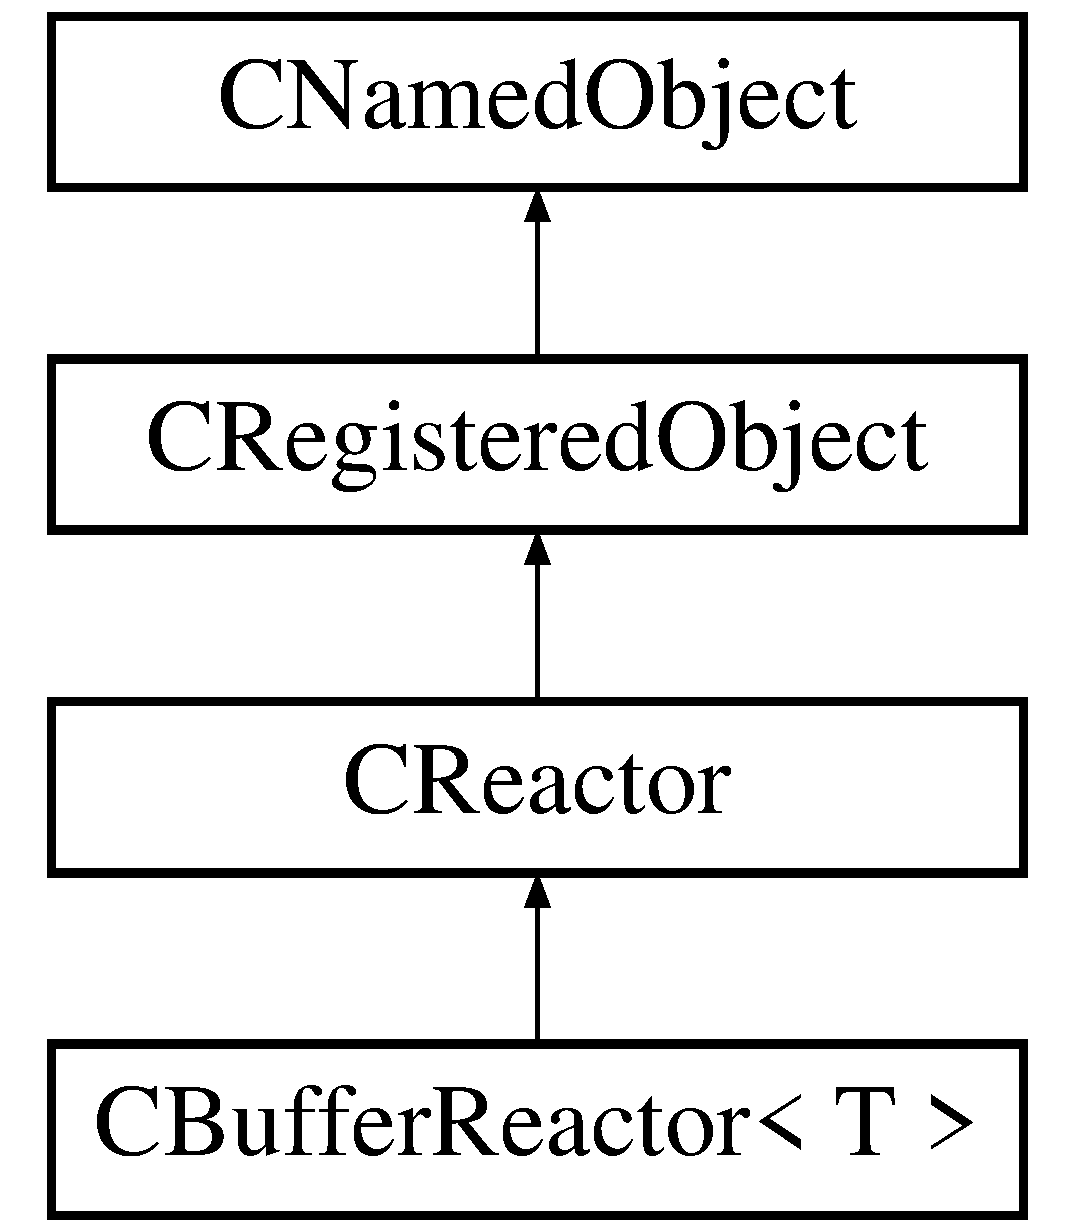
\includegraphics[height=4cm]{classCBufferReactor}
\end{center}
\end{figure}
\subsection*{Public Methods}
\begin{CompactItemize}
\item 
{\bf CBuffer\-Reactor} ()
\item 
{\bf CBuffer\-Reactor} (const string \&r\-Name)
\item 
{\bf CBuffer\-Reactor} (const char $\ast$p\-Name)
\item 
{\bf $\sim$CBuffer\-Reactor} ()
\item 
template$<$class U$>$ int {\bf operator==} (const CBuffer\-Reactor$<$ U $>$ \&a\-CBuffer\-Reactor) const
\begin{CompactList}\small\item\em Operator== Equality comparison:.\item\end{CompactList}\item 
virtual void {\bf On\-Event} ({\bf CEvent\-Monitor} \&r\-Monitor)
\item 
virtual void {\bf On\-Buffer} ({\bf CBuffer\-Monitor}$<$ T $>$ \&r\-Monitor, Pointer$<$ DAQBuffer$<$ T $>$, T $>$ p\-Buffer)
\end{CompactItemize}
\subsection*{Private Methods}
\begin{CompactItemize}
\item 
{\bf CBuffer\-Reactor} (const CBuffer\-Reactor \&a\-CBuffer\-Reactor)
\begin{CompactList}\small\item\em Copy Constructor disallowed.\item\end{CompactList}\item 
CBuffer\-Reactor \& {\bf operator=} (const CBuffer\-Reactor \&a\-CBuffer\-Reactor)
\begin{CompactList}\small\item\em Operator= Assignment Operator disallowed.\item\end{CompactList}\end{CompactItemize}


\subsection{Detailed Description}
\subsubsection*{template$<$class T$>$ class CBuffer\-Reactor$<$ T $>$}

Base class for Spectro\-Daq buffer receipt. This object must be subclassed to provide application specific processing. 



Definition at line 327 of file CBuffer\-Reactor.h.

\subsection{Constructor \& Destructor Documentation}
\index{CBufferReactor@{CBuffer\-Reactor}!CBufferReactor@{CBufferReactor}}
\index{CBufferReactor@{CBufferReactor}!CBufferReactor@{CBuffer\-Reactor}}
\subsubsection{\setlength{\rightskip}{0pt plus 5cm}template$<$class T$>$ CBuffer\-Reactor$<$ T $>$::CBuffer\-Reactor ()}\label{classCBufferReactor_a0}


Construct a buffer reactor with a default name. Note that buffer reactors are templated by the type of data contained in the buffer. 

Definition at line 310 of file CBuffer\-Reactor.cpp.

References CNamed\-Object::Append\-Class\-Info().\index{CBufferReactor@{CBuffer\-Reactor}!CBufferReactor@{CBufferReactor}}
\index{CBufferReactor@{CBufferReactor}!CBufferReactor@{CBuffer\-Reactor}}
\subsubsection{\setlength{\rightskip}{0pt plus 5cm}template$<$class T$>$ CBuffer\-Reactor$<$ T $>$::CBuffer\-Reactor (const string \& {\em r\-Name})}\label{classCBufferReactor_a1}


Construct a named buffer reactor using an STL string parameter for the object name. \begin{Desc}
\item[Parameters: ]\par
\begin{description}
\item[{\em 
r\-Name}]- the name of the reactor. \end{description}
\end{Desc}


Definition at line 322 of file CBuffer\-Reactor.cpp.

References CNamed\-Object::Append\-Class\-Info().\index{CBufferReactor@{CBuffer\-Reactor}!CBufferReactor@{CBufferReactor}}
\index{CBufferReactor@{CBufferReactor}!CBufferReactor@{CBuffer\-Reactor}}
\subsubsection{\setlength{\rightskip}{0pt plus 5cm}template$<$class T$>$ CBuffer\-Reactor$<$ T $>$::CBuffer\-Reactor (const char $\ast$ {\em p\-Name})}\label{classCBufferReactor_a2}


Construct a named buffer reactor using a ASCIZ (C) string parameter for the object name. \begin{Desc}
\item[Parameters: ]\par
\begin{description}
\item[{\em 
p\-Name}]- Pointer to an ASCIZ string naming the buffer. \end{description}
\end{Desc}


Definition at line 334 of file CBuffer\-Reactor.cpp.

References CNamed\-Object::Append\-Class\-Info().\index{CBufferReactor@{CBuffer\-Reactor}!~CBufferReactor@{$\sim$CBufferReactor}}
\index{~CBufferReactor@{$\sim$CBufferReactor}!CBufferReactor@{CBuffer\-Reactor}}
\subsubsection{\setlength{\rightskip}{0pt plus 5cm}template$<$class T$>$ CBuffer\-Reactor$<$ T $>$::$\sim$CBuffer\-Reactor ()}\label{classCBufferReactor_a3}




Definition at line 340 of file CBuffer\-Reactor.cpp.\index{CBufferReactor@{CBuffer\-Reactor}!CBufferReactor@{CBufferReactor}}
\index{CBufferReactor@{CBufferReactor}!CBufferReactor@{CBuffer\-Reactor}}
\subsubsection{\setlength{\rightskip}{0pt plus 5cm}template$<$class T$>$ CBuffer\-Reactor$<$ T $>$::CBuffer\-Reactor (const CBuffer\-Reactor$<$ T $>$ \& {\em a\-CBuffer\-Reactor})\hspace{0.3cm}{\tt  [private]}}\label{classCBufferReactor_c0}


Copy Constructor disallowed.



\subsection{Member Function Documentation}
\index{CBufferReactor@{CBuffer\-Reactor}!OnBuffer@{OnBuffer}}
\index{OnBuffer@{OnBuffer}!CBufferReactor@{CBuffer\-Reactor}}
\subsubsection{\setlength{\rightskip}{0pt plus 5cm}template$<$class T$>$ void CBuffer\-Reactor$<$ T $>$::On\-Buffer ({\bf CBuffer\-Monitor}$<$ T $>$ \& {\em r\-Monitor}, Pointer$<$ DAQBuffer$<$ T $>$, T $>$ {\em p\-Buffer})\hspace{0.3cm}{\tt  [virtual]}}\label{classCBufferReactor_a6}


Called when a buffer has been received by a buffer monitor. In normal use, the user will subclass CBuffer\-Reactor and override this no-op member. \begin{Desc}
\item[Parameters: ]\par
\begin{description}
\item[{\em 
r\-Monitor}]- The buffer monitor which received the buffer. \item[{\em 
p\-Buffer}]- A DAQBuffer\-Ptr of the appropriate type into the buffer received. \end{description}
\end{Desc}


Reimplemented in {\bf CBuffer\-Event$<$ T $>$::CGeneric\-Buffer\-Reactor$<$ T $>$} {\rm (p.\,\pageref{classCBufferEvent_1_1CGenericBufferReactor_a1})}.

Definition at line 389 of file CBuffer\-Reactor.cpp.

Referenced by CBuffer\-Reactor$<$ T $>$::On\-Event().\index{CBufferReactor@{CBuffer\-Reactor}!OnEvent@{OnEvent}}
\index{OnEvent@{OnEvent}!CBufferReactor@{CBuffer\-Reactor}}
\subsubsection{\setlength{\rightskip}{0pt plus 5cm}template$<$class T$>$ void CBuffer\-Reactor$<$ T $>$::On\-Event ({\bf CEvent\-Monitor} \& {\em r\-Monitor})\hspace{0.3cm}{\tt  [virtual]}}\label{classCBufferReactor_a5}


Called when the event monitor declares an event. The event monitor must be descended from {\bf CBuffer\-Monitor} {\rm (p.\,\pageref{classCBufferMonitor})} or  this function will throw a {\bf CIncompatible\-Monitor} {\rm (p.\,\pageref{classCIncompatibleMonitor})} exception. The On\-Buffer virtual member is called with a pointer to the buffer. \begin{Desc}
\item[Parameters: ]\par
\begin{description}
\item[{\em 
r\-Monitor}]- Reference to the monitor which declared the event. \end{description}
\end{Desc}


Reimplemented from {\bf CReactor} {\rm (p.\,\pageref{classCReactor_a6})}.

Definition at line 365 of file CBuffer\-Reactor.cpp.

References CBuffer\-Monitor$<$ T $>$::get\-Buffer\-Pointer(), and CBuffer\-Reactor$<$ T $>$::On\-Buffer().\index{CBufferReactor@{CBuffer\-Reactor}!operator=@{operator=}}
\index{operator=@{operator=}!CBufferReactor@{CBuffer\-Reactor}}
\subsubsection{\setlength{\rightskip}{0pt plus 5cm}template$<$class T$>$ CBuffer\-Reactor\& CBuffer\-Reactor$<$ T $>$::operator= (const CBuffer\-Reactor$<$ T $>$ \& {\em a\-CBuffer\-Reactor})\hspace{0.3cm}{\tt  [private]}}\label{classCBufferReactor_c1}


Operator= Assignment Operator disallowed.

\index{CBufferReactor@{CBuffer\-Reactor}!operator==@{operator==}}
\index{operator==@{operator==}!CBufferReactor@{CBuffer\-Reactor}}
\subsubsection{\setlength{\rightskip}{0pt plus 5cm}template$<$class T$>$ template$<$class U$>$ int CBuffer\-Reactor$<$ T $>$::operator== (const CBuffer\-Reactor$<$ U $>$ \& {\em a\-CBuffer\-Reactor}) const}\label{classCBufferReactor_a4}


Operator== Equality comparison:.



Definition at line 349 of file CBuffer\-Reactor.cpp.

References CReactor::operator==().

The documentation for this class was generated from the following files:\begin{CompactItemize}
\item 
{\bf CBuffer\-Reactor.h}\item 
{\bf CBuffer\-Reactor.cpp}\end{CompactItemize}
